%-------------------------------------------------------------------------------
\chapter{Background}
\label{ch.background}
%-------------------------------------------------------------------------------

\section{Basic Terminology}
This section contains definitions of some basic terms that are used in the thesis.

{\bf Walking bipedal robots} are robotic systems that can walk using two legs. 
Terms {\bf biped}, which stands for any two-footed animal or robot; {\bf humanoid},
which denotes mechanical systems or creatures having human appearance; and {\bf walking 
bipedal robot} are used interchangeably in this thesis. 

{\bf Walking} is defined as a locomotion of a system having multiple contacts with the 
ground by means of breaking and regaining these contacts without simultaneous breaking 
of all contacts. A typical {\bf walking cycle} of a biped is shown in \cref{fig.walkcycle}.

\begin{figure}[ht]
    \centerline{%
    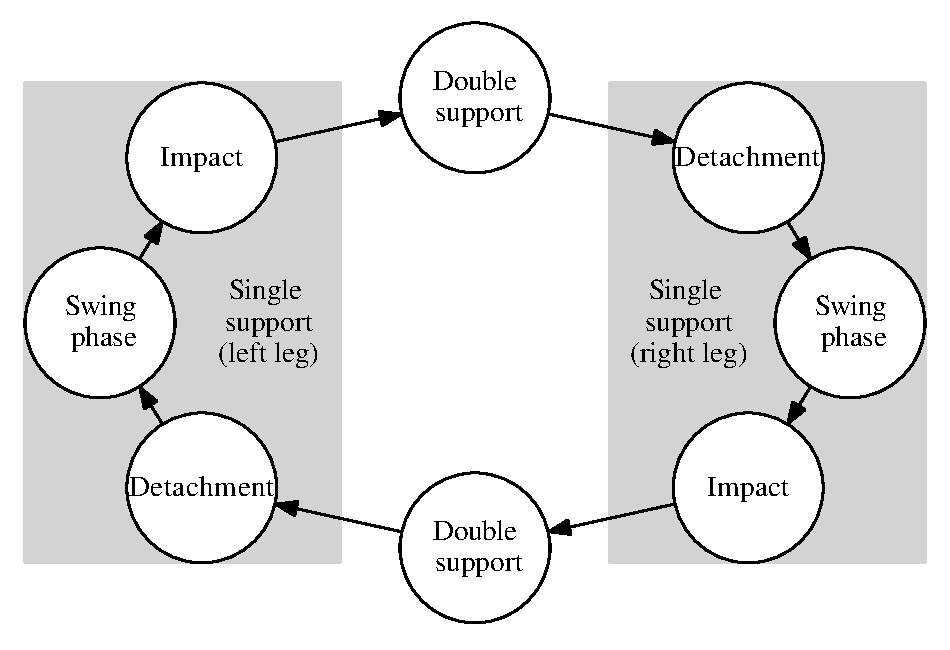
\includegraphics[scale=0.45]{Figures/walk_cycle.eps}}
    \caption[Walking cycle of a biped]{Walking cycle of a biped is typically defined in
    such a way, that it includes two swing phases of right and left leg and two phases 
    when both feet are on the ground.}
    \label{fig.walkcycle}
\end{figure}

The convex hull of the ground contacts in the ground plane is called the {\bf support area}.
In practical applications it is often represented by a polygon, hence an equivalent term 
\ac{PoS} is often used. 

The phase of the walking cycle when only one foot contact with the ground is preserved is
referred to as \ac{SS}, while the phase when both feet are in contact with the ground 
is called \ac{DS}. \ac{SS} and \ac{DS} are also used to denote the respective support area.

{\bf Step} is defined as a half of walking cycle, which includes one single support 
and adjacent double support. {\bf Footstep} denotes the position of a foot in ground plane.
The term ``gait'' is used to denote a pattern of movements of a robot during walk.

In accordance with \cite{VukHumanoidTerms} {\bf balance} is defined as the state, in which 
humanoid preserves the upright position. Some authors use the word ``stability'' instead of 
``balance'', but such use is avoided here to prevent confusion. Terms {\bf static balance} 
and {\bf dynamic balance} are used to discriminate situations when a robot is balanced
while it is still, and while it is moving. The ability to preserve balance is a crucial 
characteristic for walking robots. 


%%%%%%%%%%%%%%%%%%%%%%%%%%%%%%%%%%%%%%%%%%%%%%%%%%%%%%%%%%%%%%%%%%%%%%%%%%%%%%%%
%%%%%%%%%%%%%%%%%%%%%%%%%%%%%%%%%%%%%%%%%%%%%%%%%%%%%%%%%%%%%%%%%%%%%%%%%%%%%%%%
%%%%%%%%%%%%%%%%%%%%%%%%%%%%%%%%%%%%%%%%%%%%%%%%%%%%%%%%%%%%%%%%%%%%%%%%%%%%%%%%
\section{Dynamic Balance}
The dynamic balance of a biped can be ensured using one of the criteria presented
in this section. Note that it is possible to design a gait, which is not balanced
with respect even to the most general criteria mentioned here. For example, a gait
may include a phase of controlled fall, when the fall is started intentionally and 
appropriate preparations are made in order to continue the walk after the foot impact.
Nevertheless, design of such gaits is not a trivial task.

Also, there is a class of robots, which are designed using a completely different
paradigm. Continuous walk of such robots is characterized by a cycle in the phase 
plane, which is supported either naturally or using control \cite{KajitaLegged}. 
{\bf Passive walkers}, which were introduced in \cite{McGeer}, are the best known 
representatives of this class of systems. Walking is a natural dynamic mode of 
passive walkers. Their mechanical design allows them to walk on shallow slopes 
without any active control. Combination of passive dynamics with actuation is also 
a promising research direction \cite{CollinsPassive}. 
% TODO The main disadvantage of the current passive walkers is the lack of agility and responsiveness.


%%%%%%%%%%%%%%%%%%%%%%%%%%%%%%%%%%%%%%%%%%%%%%%%%%%%%%%%%%%%%%%%%%%%%%%%%%%%%%%%
\subsection{Center of Mass}
One of the best known balance criteria is the position of the projection of the \ac{CoM} 
on the ground plane, which must stay within the support area. This criterion was used in 
other engineering disciplines before it was adopted in robotics. Robots that balance 
using projection of \ac{CoM} are called {\bf static walkers} to indicate, that the 
static balance is always preserved. Hence, they can be safely stopped at any moment.

Static walkers are rather limited in their capabilities, in particular their walk is 
rather slow, since they must limit their acceleration. Note that this criterion is 
valid only when all ground contacts of a robot lie on the same horizontal plane 
\cite{WieberStability}.


%%%%%%%%%%%%%%%%%%%%%%%%%%%%%%%%%%%%%%%%%%%%%%%%%%%%%%%%%%%%%%%%%%%%%%%%%%%%%%%%
\subsection{Zero Moment Point}
This criterion, which is based on the existence of \ac{ZMP} \cite{VukZMP35}, was 
proposed by Miomir Vukobratovi\'c in $1968$ at the Third All-Union Congress on 
Theoretical and Applied Mechanics in Moscow. 

The concept of \ac{ZMP} is introduced under the assumption that a robot walks on a flat
floor and the friction forces are strong enough to compensate the ground reaction
forces tangential to the ground.

Since the ground contact of a robot is unilateral (the robot can push on the ground, 
but cannot pull), the only force that can compensate forces that tend to overturn the 
robot is the ground reaction force. The point where the ground reaction force must be 
applied to compensate for other forces must exist within the support area, otherwise 
the robot would lose balance. This point is named \ac{ZMP}.

When the \ac{ZMP} does not exist within the support area, under the assumption that the
support is immobile (which is not true in this case) a \ac{FZMP} can be found in order 
to measure the disbalance \cite{VukHumanoidTerms}.

The position of \ac{CoP}, which is a a point on the ground plane, where the ground 
reaction force is applied, is often considered to be an equivalent of \ac{ZMP}, since they 
coincide while the robot is balanced. Therefore, the actual position of \ac{ZMP} can be 
found using force sensors located on the soles of a robot.

Even though the situation when \ac{ZMP} exists on the edge of the support area do not
necessary lead to fall, it is dangerous since any small disturbance may overturn
the robot. The easiest way to avoid this is to define support area with a safety 
margin.


%%%%%%%%%%%%%%%%%%%%%%%%%%%%%%%%%%%%%%%%%%%%%%%%%%%%%%%%%%%%%%%%%%%%%%%%%%%%%%%%
\subsection{Other Criteria}
The forenamed criteria cannot be used on uneven terrain, but a more general criteria
can be developed \cite{WieberStability, BretlEquilibrium, AdiosZMP}. Nevertheless,
they are computationally more expensive and may be infeasible for real-time applications
\cite{WieberStability}. 

%Some authors have also extended \ac{ZMP} heuristically \cite{SardainZMP}.



%%%%%%%%%%%%%%%%%%%%%%%%%%%%%%%%%%%%%%%%%%%%%%%%%%%%%%%%%%%%%%%%%%%%%%%%%%%%%%%%
%%%%%%%%%%%%%%%%%%%%%%%%%%%%%%%%%%%%%%%%%%%%%%%%%%%%%%%%%%%%%%%%%%%%%%%%%%%%%%%%
%%%%%%%%%%%%%%%%%%%%%%%%%%%%%%%%%%%%%%%%%%%%%%%%%%%%%%%%%%%%%%%%%%%%%%%%%%%%%%%%
\section{3D Linear Inverted Pendulum Model}\label{sec.3dlipm}
Apart from balancing there are other factors that complicate control of walking
robots. Hence, it is common to make simplifying assumptions. For example, in this
thesis it is assumed that walk is performed in such a way, that constraints 
imposed by environment, joint limits, self-collision avoidance are never violated.

However, it is necessary to make other assumptions. Consider generation of trajectories
for a humanoid in the joint or operational space. If these trajectories are generated
offline, the motion cannot adapt to the walk conditions. Hence, it is more appealing to 
generate motion profiles online. This can be achieved with the help of \ac{MPC} 
\cite{KajitaLegged}, refer to \cref{ch.MPC} for more information on \ac{MPC}. If the whole 
model of a robot robot is incorporated in the \ac{MPC}, then the respective optimization 
problem becomes nonlinear \cite{KajitaLegged}. Real-time control based on \ac{NMPC} is 
not always feasible, since its application is a computationally expensive task. This 
limitation motivated researchers to develop control schemes that avoid \ac{NMPC} and 
use simple \ac{LMPC} instead.

The dynamics of a humanoid walking on a flat ground can be approximated (in a reasonable 
way) by a linear model, which is called \ac{3D-LIPM} \cite{3d-lipm}. This model is based 
on two important assumptions. The first one allows to ignore the structure of the robot 
in order to represent it by an inverted pendulum. The second one restricts motions of 
pendulum to a plane in order to obtain linear model. Though, this plane can be inclined, 
henceforth it is assumed to be parallel to the ground surface and intersect the $z$ axis
at the height of \ac{CoM} $c^z$.

The \ac{3D-LIPM} system must be controlled using torques. For convenience, the torques
can be expressed through the coordinates of \ac{ZMP} leading to {\bf cart-on-a-table 
model} \cite{LIPM-MPC}. This model allows computation of \ac{ZMP} position using
\begin{equation}\label{eq.zmp_cart}
\begin{split}
z^x &= c^x - h \ddot{c}^x, \\
z^y &= c^y - h \ddot{c}^y, \\
\end{split}
\end{equation}
where 
$$
h = \frac{c^z}{g};
$$
$(z^x, z^y)$ and $(c^x, c^y)$ are coordinates of \ac{ZMP} and \ac{CoM} on the 
horizontal plane; $(\ddot{c}^x, \ddot{c}^y)$ are the accelerations of \ac{CoM} 
on the horizontal plane; $g = 9.8$ is gravitational acceleration; $c^z$ is the height
of the plane, in which motion of the \ac{CoM} is constrained.

Based on the \cref{eq.zmp_cart} a discrete-time time-invariant linear dynamical 
system can be obtained using trivial integration
\begin{equation}\label{eq.system_orig}
\begin{split}
\hat{\mbm{c}}_{k+1} &= \mbm{A}\hat{\mbm{c}}_{k}+\mbm{B}\dddot{\mbm{c}}_{k}\\
\mbm{z}_k &= \mbm{C} \hat{\mbm{c}}_{k}.
\end{split}
\end{equation}
Where the state
$$
\hat{\mbm{c}}_{k} = 
\begin{bmatrix} 
c_k^x & \dot{c}_k^x & \ddot{c}_k^x & c_k^y & \dot{c}_k^y & \ddot{c}_k^y
\end{bmatrix}^T
$$
includes the position, velocity, and acceleration of \ac{CoM}; and the control
vector
$$
\dddot{\mbm{c}}_{k} = \begin{bmatrix} \dddot{c}_k^x & \dddot{c}_k^y \end{bmatrix}^T;
$$
consists of jerks of \ac{CoM}.
State transition and control input matrices are
$$
\mbm{A} = 
\begin{bmatrix}
    1 & T & T^{2}/2 & 0 & 0 & 0\\ 
    0 & 1 & T & 0 & 0 & 0\\ 
    0 & 0 & 1 & 0 & 0 & 0\\
    0 & 0 & 0 & 1 & T & T^{2}/2\\
    0 & 0 & 0 & 0 & 1 & T\\
    0 & 0 & 0 & 0 & 0 & 1
\end{bmatrix}, \quad
\mbm{B} =
\begin{bmatrix}
    T^{3}/6 & 0\\ 
    T^{2}/2 & 0\\
    T      & 0\\
    0      & T^{3}/6\\
    0      & T^{2}/2\\
    0      & T
\end{bmatrix},
$$
where $T$ is the length of a discretization step in seconds; and the output matrix is
$$
\mbm{C} = 
\begin{bmatrix}
    1 & 0 & -h & 0 & 0 & 0\\ 
    0 & 0 & 0  & 1 & 0 & -h\\
\end{bmatrix}.
$$
The system~\eqref{eq.system_orig} is suitable for implementation of an \ac{MPC} 
controller for \ac{CoM} and \ac{ZMP} trajectory generation. 

Another approach to generation of these trajectories is based on analytical 
solutions of the differential equations~\eqref{eq.zmp_cart}, for example refer to 
\cite{MorisawaAnalytical,LiuAnalytical}. In this case the \ac{ZMP} trajectory 
can be represented by a polynomial. 
%This approach can be preferrable in situations,
%when the future footsteps are not known. When \ac{MPC} scheme is used, at least
%several footsteps must be defined in advance (the reason is explained in 
%\cref{sec.mpc_stability}).


%%%%%%%%%%%%%%%%%%%%%%%%%%%%%%%%%%%%%%%%%%%%%%%%%%%%%%%%%%%%%%%%%%%%%%%%%%%%%%%%
%%%%%%%%%%%%%%%%%%%%%%%%%%%%%%%%%%%%%%%%%%%%%%%%%%%%%%%%%%%%%%%%%%%%%%%%%%%%%%%%
%%%%%%%%%%%%%%%%%%%%%%%%%%%%%%%%%%%%%%%%%%%%%%%%%%%%%%%%%%%%%%%%%%%%%%%%%%%%%%%%
\section{Nao Overview}\label{sec.nao}
The experimental part of this thesis was conducted on a Nao robot. A software 
module developed for control of this robot is described in \cref{ch.naomodule}.

\begin{figure}[ht]
    \centerline{%
    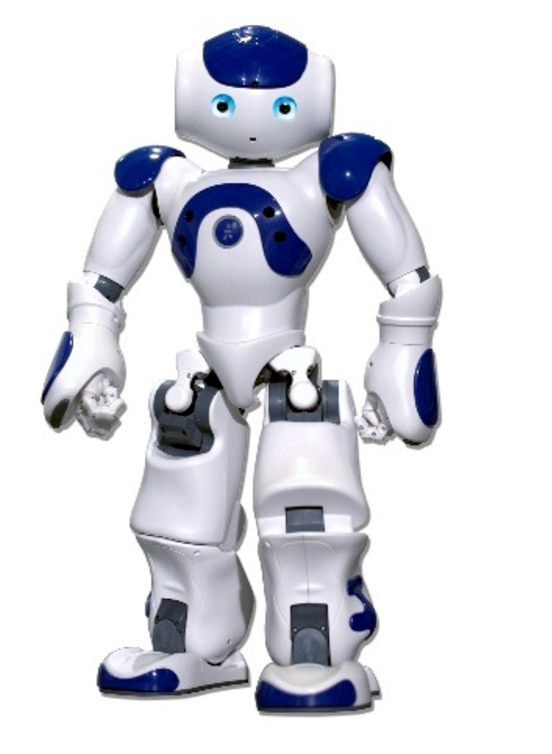
\includegraphics[scale=0.35]{Figures/nao.eps}}
    \caption[The Nao robot]{The Nao robot. The walking pattern generator that was 
    developed during the work on the thesis was tested on a Nao robot.}
    \label{fig.nao}
\end{figure}
Nao (see \cref{fig.nao}) is a small, fully actuated, position-controlled humanoid 
robot developed by a french company Aldebaran Robotics. We are working with 
version $3.2$ of this robot, which is $58$ centimeters tall, weights about $4.5$ 
kilograms and has $25$ degrees of freedom. The parameters of the processor installed
on this version of Nao is given in \cref{tbl.cpu}.

\begin{table}
\begin{center}
\begin{tabular}{c|p{7cm}}
model name & Geode(TM) Integrated Processor by AMD PCS\\
cpu MHz    & 499.903\\
cache size & 128 KB\\
flags      & fpu de pse tsc msr cx8 sep pge cmov clflush
             mmx mmxext 3dnowext 3dnow\\
\end{tabular}
\caption[The Nao CPU information]{The Nao CPU information.}
\label{tbl.cpu}
\end{center}
\end{table}

The operating system of the Nao robots is based on Linux. Various functionalities 
of Nao are provided by modules, which run within \verb|NaoQI| framework on Nao or 
a computer. Modules communicate with each other transparently through special 
application programming interface. \verb|NaoQI| framework supports modules written 
in \verb|C++| or \verb|python|. In order to build modules that must run on the
robot, the \ac{SDK} is required. The fresh releases of the operating system, the 
\ac{SDK}, and a comprehensive documentation\footnote{The Nao software documentation 
is available on the website of Aldebaran Robotics at
\url{http://www.aldebaran-robotics.com/documentation/index.html}.}
can be obtained from Aldebaran Robotics. The version of \ac{SDK} and operating system, 
which were used for development and tests, is $1.12$.

The standard software distribution for the Nao robots includes a walking module,
which uses the control scheme described in \cite{NaoWalk}.
